\chapter{Methodology}
\label{chap:met}
\chaptermark{Third Chapter Heading}

Chapter overview

% \section{Compilers and evm theory}
% \label{}

% \subsection{Introduction to compilers}

% Compiler construction is a sophisticated field in computer science, involving the creation of software that translates source code written in a high-level programming language into a lower-level language, often machine code. The process of compiler construction is typically divided into several distinct phases, each with its specialized function:


% \begin{enumerate}
%     \item Lexical Analysis
%           \begin{itemize}
%               \item Token Generation: The compiler's first phase involves breaking down the source code into tokens, which are the basic building blocks of the language (like keywords, operators, identifiers, literals).
%               \item Regular Expressions: Lexical analyzers often use regular expressions to recognize these tokens, simplifying the source code into a stream of tokens for further processing.
%           \end{itemize}

%     \item Syntax Analysis
%           \begin{itemize}
%               \item Parsing: This phase involves analyzing the token sequence from lexical analysis to ensure that the expressions and statements conform to the rules of the programming language's grammar.
%               \item Syntax Trees: The result is often a syntax tree, which represents the syntactic structure of the source code in a hierarchical tree format.
%           \end{itemize}
%     \item Semantic Analysis
%           \begin{itemize}
%               \item Type Checking: The compiler checks whether the parsed code makes logical sense, adhering to the language's semantic rules. This includes type checking, where the compiler verifies that each operation is compatible with its operands.
%               \item Symbol Table: The compiler uses a symbol table to keep track of variable names, their types, and other relevant information to ensure correct interpretation and context.
%           \end{itemize}
%     \item Intermediate Code Generation
%           \begin{itemize}
%               \item Abstract Representation: The compiler translates the source code into an intermediate representation, which is a lower-level representation of the program that retains its logical structure.
%               \item Platform-Independent Code: This intermediate code is typically platform-independent, serving as a bridge between the high-level source code and the machine code.
%           \end{itemize}
%     \item Optimization
%           \begin{itemize}
%               \item Performance Improvement: The optimization phase refines the intermediate code to improve efficiency and performance. This can include eliminating redundant calculations, optimizing loops, and more.
%               \item Target-Dependent Optimizations: These optimizations often vary depending on the target machine's architecture and capabilities.
%           \end{itemize}
%     \item Code Generation
%           \begin{itemize}
%               \item Machine Code: The final phase involves translating the optimized intermediate code into machine code specific to the target machine CPU architecture or virtual machine instruction set.
%               \item Assembly Language: Sometimes, the output is in the form of assembly language, which is then further translated into machine code by an assembler.
%           \end{itemize}
%     \item  Linking and Loading
%           \begin{itemize}
%               \item Linking: If the program consists of multiple source code files or external libraries, the linking process combines these into a single executable.
%               \item Loading: The loader then places the executable into memory for execution by the machine.
%           \end{itemize}
% \end{enumerate}

% In the context of Elixireum, these compiler construction principles must be adapted to suit the specific needs of the Ethereum Virtual Machine (EVM). This includes considerations for smart contract compilation, optimization for gas efficiency, and adhering to the deterministic execution model of the EVM. Understanding these compiler construction phases is essential for Elixireum development, as each stage plays a critical role in transforming high-level Elixireum code into efficient, secure, and EVM-compatible bytecode.

% \subsection{Ethereum Virtual Machine - A Deeper Insight}

% EVM is a core component of the Ethereum blockchain, pivotal in maintaining its decentralized and secure nature. It serves as an execution environment for smart contracts, enabling the remarkable functionality that Ethereum offers. Understanding the EVM is crucial for developing Elixireum, as it provides the foundational framework within which this new language operates.

% \begin{enumerate}
%     \item  Execution Environment
%           \begin{itemize}
%               \item Isolated System: The EVM operates as an isolated environment, completely sandboxed from the Ethereum network. This isolation ensures that code execution within the EVM does not directly affect the network or the filesystem of the host computer.
%               \item Deterministic Execution: The EVM is designed to be deterministic. This means that executing the same smart contract with the same input will always produce the same output across all nodes in the Ethereum network. This characteristic is essential for maintaining consistency and agreement (consensus) across the decentralized network.
%           \end{itemize}
%     \item EVM's Role in Smart Contracts
%           \begin{itemize}
%               \item Smart Contract Lifecycle: Developers write smart contracts in high-level languages like Solidity or Vyper. These contracts are then compiled into EVM bytecode. When a contract is deployed on the Ethereum blockchain, it's executed by the EVM to ensure it behaves as expected.
%               \item           Gas Mechanism: The EVM uses a gas mechanism to measure and limit the resources (computation and storage) a contract can use. Each operation in the EVM has a gas cost associated with it, preventing inefficient or malicious code from overloading the network.
%           \end{itemize}
%     \item State Machine
%           \begin{itemize}
%               \item           State Transitions: The EVM can be viewed as a state machine, where transactions transition the Ethereum blockchain from one state to another. Smart contracts, through their executions, modify the state stored in the Ethereum blockchain.
%               \item           EVM Bytecode: The EVM interprets a series of bytes (bytecode) which instruct the machine on the operations to perform. This bytecode is the compiled version of high-level contract code.
%           \end{itemize}
%     \item Storage and Memory
%           \begin{itemize}
%               \item   Storage: The EVM has a long-term storage model, where data is stored persistently on the blockchain. This storage is expensive but necessary for maintaining the state across transactions.
%               \item         Memory: The EVM also includes a volatile memory space, cleared after each transaction, used for temporary storage during contract execution.
%           \end{itemize}
%     \item Challenges and Considerations for Elixireum
%           \begin{itemize}
%               \item Gas Optimization: Given the cost implications of EVM operations, Elixireum must focus on gas optimization during the compilation process.
%               \item Security and Determinism: Security vulnerabilities in smart contracts can be costly. Hence, Elixireum needs to ensure robust security measures. Additionally, the deterministic nature of the EVM requires that Elixireum-generated bytecode behaves consistently across all executions.
%           \end{itemize}



% \end{enumerate}


\section{Problems}
\label{sec:problems}

Given the unique syntax borrowed from Elixir for the language we developed, our journey in crafting Elixireum often led us to delve into the implementation of Elixir itself. Due to Elixir's niche popularity, resources on writing a compiler in Elixir are scarce, and at times, completely nonexistent on the internet. Consequently, we found ourselves independently sourcing this information, relying heavily on the original codebase, experimentation, and our accumulated expertise.
Similarly, our encounter with the intermediate Yul language presented its own set of challenges. The entirety of its documentation seems to be condensed into a single chapter within the Solidity documentation, leading to a notable dearth of practical usage examples and detailed explanations of certain concepts. Faced with these constraints, we embarked on a quest for knowledge through hands-on experimentation and meticulous analysis of the opcodes found within the bytecodes of various examples. This approach allowed us to uncover and understand the intricacies of Yul, despite the limited resources at our disposal.

\section{Design and implementations}
\label{sec:design}

This section outlines the principal elements of the Elixireum compiler's design, focusing specifically on the methodology employed to compile Elixireum code into EVM bytecode. It overviews the technology stack employed in the development process and underscores the pivotal decisions that shaped the architecture of the compiler.


\subsection{Choice of Elixir}
\begin{itemize}
    \item The rationale for selecting Elixir is straightforward: our team possesses substantial expertise in this programming language.
    \item Elixir is open source so we can easily reuse its machinery for tokenization and parsing Elixireum.
\end{itemize}

\subsection{Choice of Yul}
\begin{itemize}
    \item Initially, our strategy entailed compiling Elixireum directly into Ethereum Virtual Machine (EVM) bytecode. Subsequently, we pivoted towards an intermediate representation (IR), selecting Yul as IR aligned with our requirements. Advantages from this decision encompass:
          \begin{itemize}
              \item Compatibility with all EVM versions, obviating the need for version-specific concerns.
              \item Avoidance of reimplementing primitives such as function calls, variable and stack management, thereby freeing up resources to enhance the feature set of the language.
              \item Reduced gas consumption facilitated by the ability to optimize Yul code of Solidity compiler.
          \end{itemize}
    \item Despite these considerations, the choice comes with limitations, notably:
          \begin{itemize}
              \item Dependency on the Solidity compiler for Elixireum.
          \end{itemize}

          No significant downsides compared to direct compilation to EVM bytecode, as bytecode can be used in Yul directly.
    \item We considered the mapping of BEAM (Erlang VM) bytecode to EVM bytecode as an option as well. This option was deemed challenging due to the fundamental architectural and philosophical differences between the two virtual machines. BEAM is specifically tailored for environments that demand high concurrency, distribution, and fault tolerance, boasting a set of opcodes optimized for these conditions. In contrast, the EVM is built to run smart contracts within blockchain ecosystems, prioritizing deterministic execution and gas metering to safeguard against spam and enhance the security of the network. Due to these distinct focuses, BEAM incorporates specialized instructions for concurrency and distributed processing, which do not directly translate to EVM's capabilities.
\end{itemize}


\begin{figure}[h!]
    \centering
    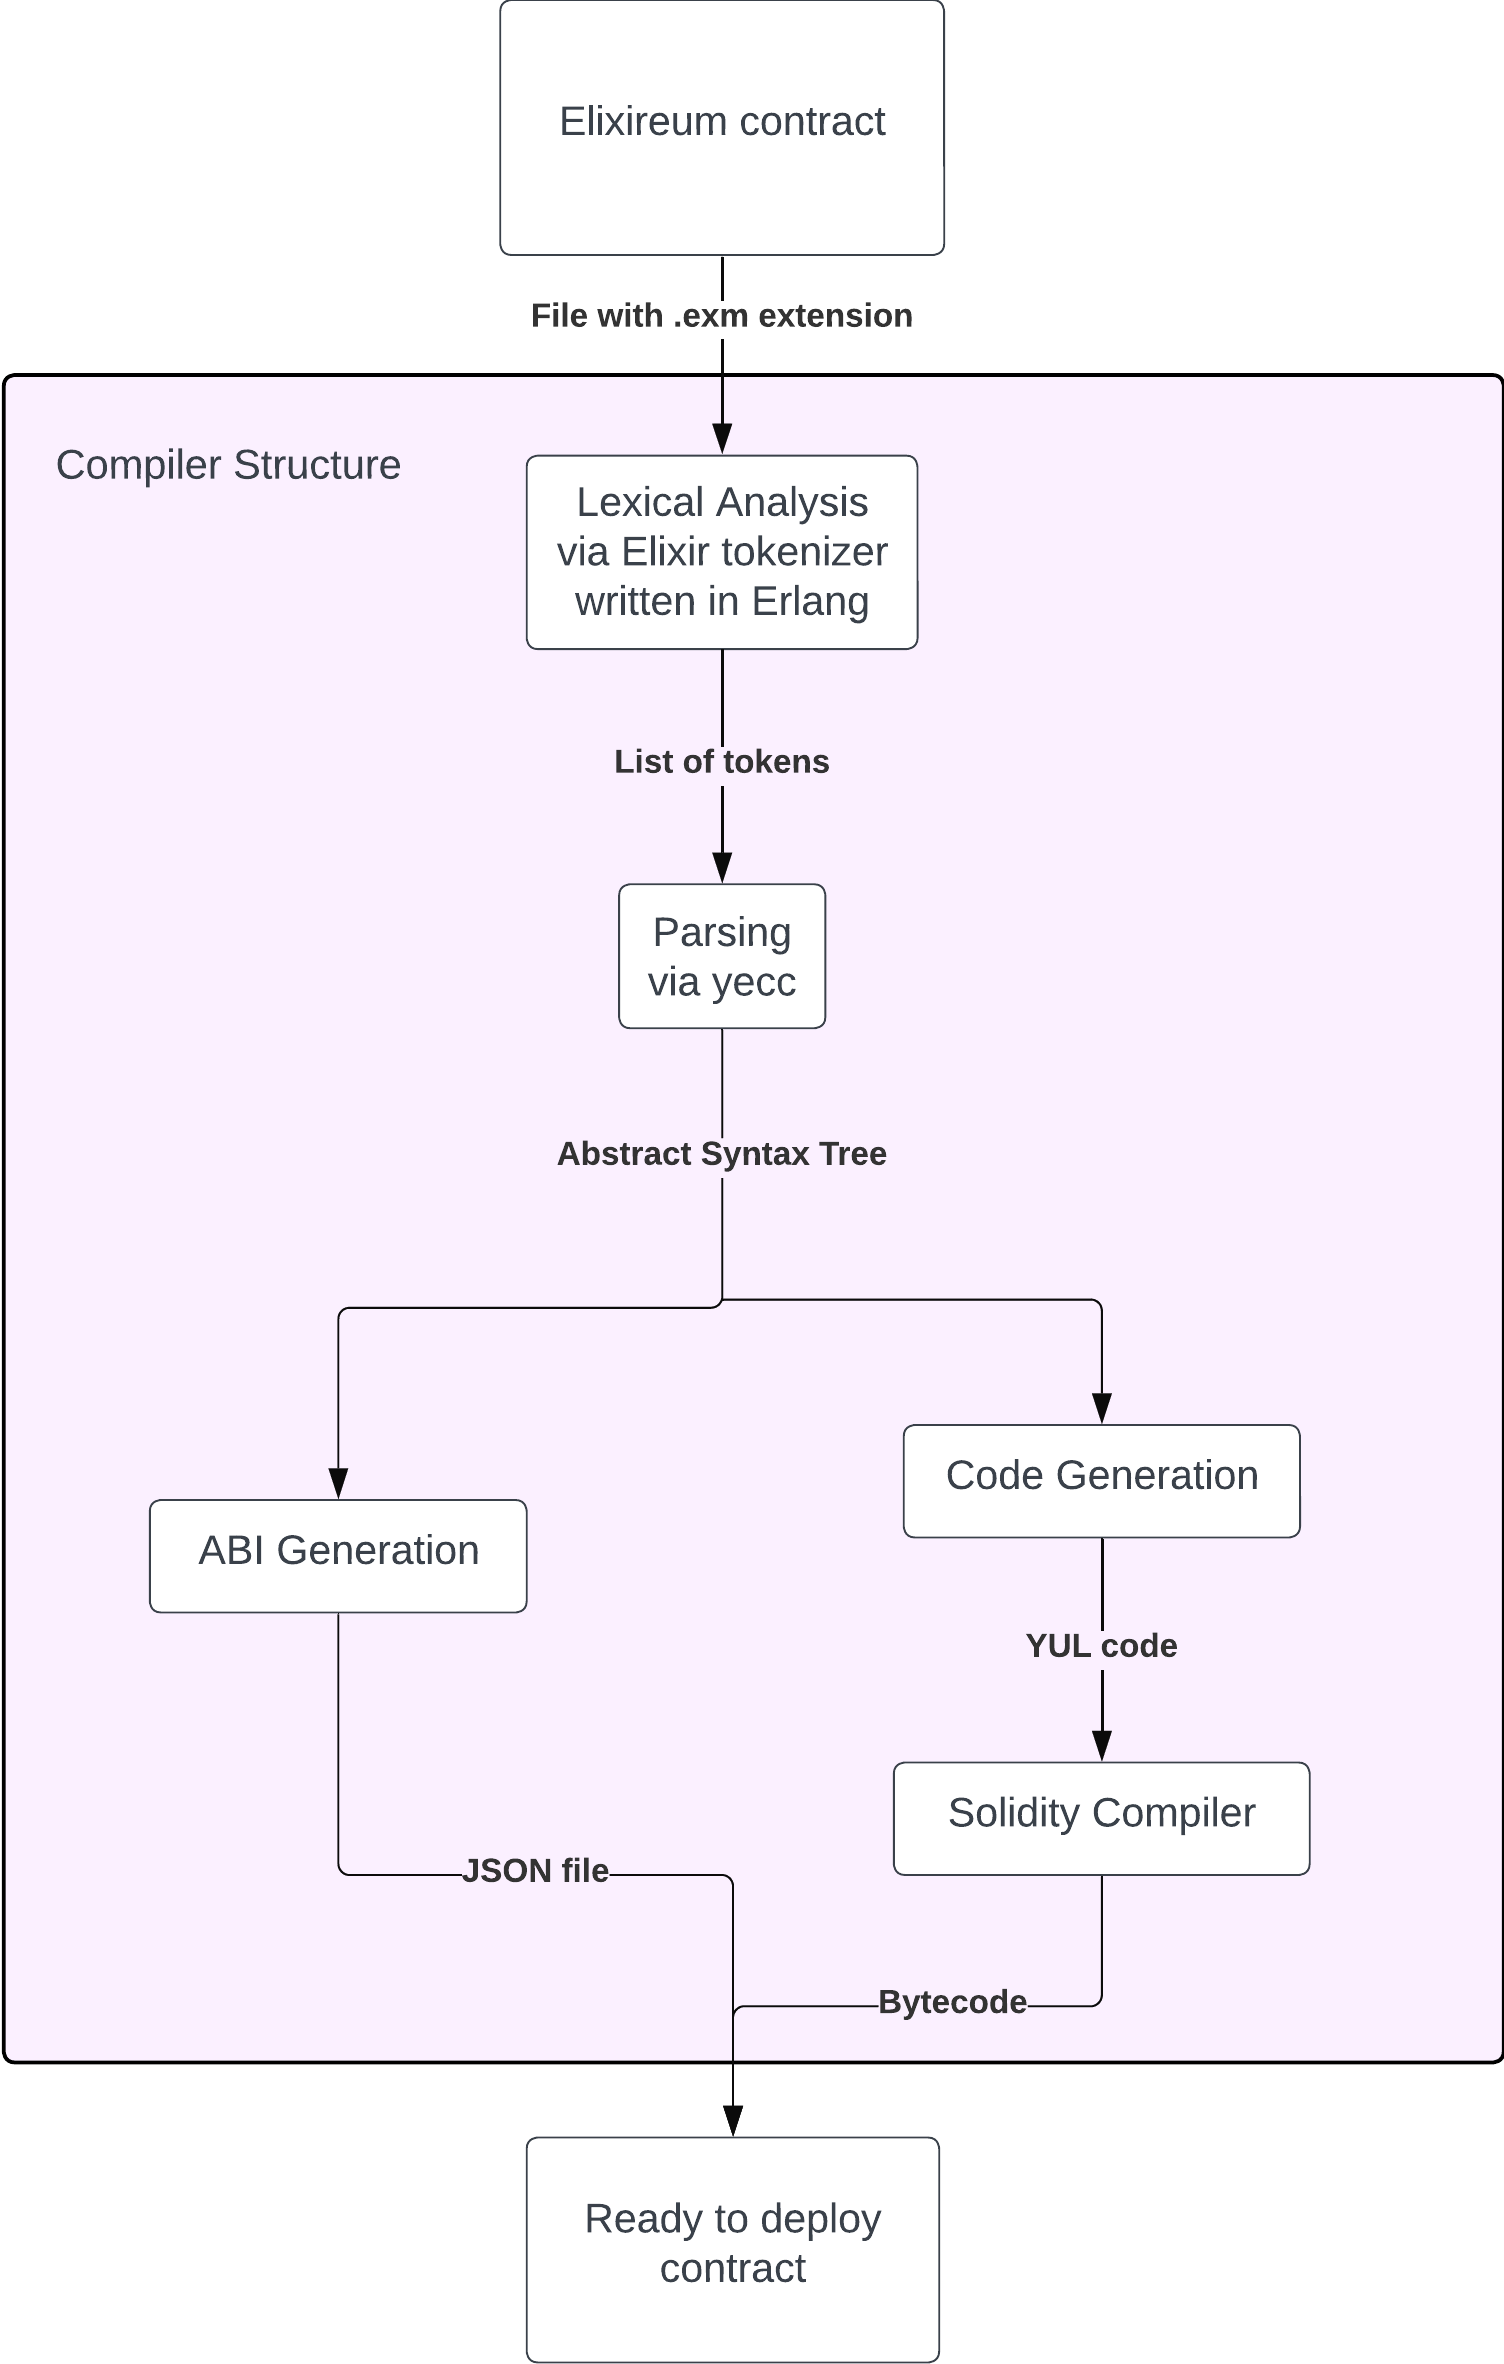
\includegraphics[width=0.8\textwidth]{figs/arch.png}
    \caption{Elixireum compiler architecture}
    \label{fig:arch}
\end{figure}

% \section{Limitations (elixirish distribution is not applicable to evm, so it is cannot be used in smart contracts, libraries are out of the scope, external smart contract interactions, need to spec types for public functions, need of solidity compiler )}
% \label{}
% NOT LIMITATIONS BUT CONSTRAINTS (OR FROM LEVS PAPER MB REQUEIREMENTS)
% While this study provides valuable insights into the application of elixirish distribution in Ethereum Virtual Machine (EVM) environments, it is important to acknowledge several limitations that may impact the generalizability and scope of the findings.

% While we

% Inapplicability to EVM:
% The elixirish distribution, a key focus of this research, is not directly applicable to the Ethereum Virtual Machine (EVM). As a result, its usage in smart contracts within the EVM environment is not feasible, limiting the direct implementation of elixirish distribution in Ethereum-based decentralized applications.

% Exclusion of Libraries:
% The scope of this study does not encompass the incorporation of external libraries. The exclusion of libraries may affect the versatility of the proposed methods, as the integration of additional functionalities from external sources is not considered in the current framework.

% External Smart Contract Interactions:
% Interactions with external smart contracts fall outside the purview of this research. The study primarily focuses on the internal dynamics and distribution mechanisms within a single smart contract. External interactions, if any, are not explored in this context.

% Specification Requirements for Public Functions:
% The necessity to specify types for public functions is a limitation inherent in the proposed methodology. While this ensures a higher degree of predictability and security, it imposes additional constraints on developers, requiring explicit type specifications for public functions to ensure compatibility with elixirish distribution.

% Dependency on Solidity Compiler:
% The reliance on the Solidity compiler is another limitation of the methods presented in this study. Changes in the Solidity language or compiler versions may impact the applicability and stability of the elixirish distribution approach, necessitating careful consideration and potential adjustments in future developments.

% It is crucial for future researchers and practitioners to be aware of these limitations when applying or extending the proposed methods in different contexts. Addressing these constraints may pave the way for more comprehensive and robust solutions in the evolving landscape of smart contract development and blockchain technologies.

% \section{other languages comparison}
% \label{}

% lorem ipsum


% \section{Conclusion}

% lorem ipsum



% \ldots

% Referencing other chapters \ref{chap:lr}, \ref{chap:met}, \ref{chap:impl}, \ref{chap:eval} and \ref{chap:conclusion}
% \begin{longtable}{c|c}
%     \caption[This is the title I want to appear in the List of Tables]{Simulation Parameters} \label{table:thisimulation_params} \\
%     \hline
%     A                                     & B                                                                                    \\
%     \hline
%     \endfirsthead
%     \multicolumn{2}{@{}l}{}                                                                                                      \\
%     \hline
%     A                                     & B                                                                                    \\
%     \hline
%     \endhead
%     \hline
%     \textbf{Parameter}                    & \textbf{Value}                                                                       \\
%     \hline
%     Number of vehicles                    & $|\mathcal{V}|$                                                                      \\
%     \hline
%     Number of RSUs                        & $|\mathcal{U}|$                                                                      \\
%     \hline
%     RSU coverage radius                   & 150 m                                                                                \\
%     \hline
%     V2V communication radius              & 30 m                                                                                 \\
%     \hline
%     Smart vehicle antenna height          & 1.5 m                                                                                \\
%     \hline
%     RSU antenna height                    & 25 m                                                                                 \\
%     \hline
%     Smart vehicle maximum speed           & $v_{max}$ m/s                                                                        \\
%     \hline
%     Smart vehicle minimum speed           & $v_{min}$ m/s                                                                        \\
%     \hline
%     Common smart vehicle cache capacities & $[50, 100, 150, 200, 250]$ mb                                                        \\
%     \hline
%     Common RSU cache capacities           & $[5000,1000,1500,2000,2500]$ mb                                                      \\
%     \hline
%     Common backhaul rates                 & $[75, 100, 150]$ mb/s                                                                \\
%     \hline
% \end{longtable}

% \begin{figure}[hbt]
%     \centering
%     
\includegraphics[]{figs/inno.png}
%     \caption{One kernel at $x_s$ (\emph{dotted kernel}) or two kernels at
%         $x_i$ and $x_j$ (\textit{left and right}) lead to the same summed estimate
%         at $x_s$. This shows a figure consisting of different types of
%         lines. Elements of the figure described in the caption should be set in
%         italics, in parentheses, as shown in this sample caption.}
%     \label{fig:thiex}
% \end{figure}


% \ldots